\subsection{Fringing}
\label{fringe:main}


The major causes for fringing are the night sky emission lines (mainly
OH transition) in the upper atmosphere. If monochromatic lines are
reflected within the CCD they interfere producing a fringe-pattern
(usually variable over night). Some instruments show considerable
fringing in certain wavebands like the z-band. To correct for the
latter a master fringe image has to be created and subtracted before
doing photometric measurements.

\subsubsection{Master fringe computation}
\label{fringe:algorithms:compute}

This algorithm extracts a master fringe from a sequence of images.


\paragraph{Algorithm - short description}
\label{fringe:algorithms:compute:short}


The algorithm consists of two main steps: i) Using a Gaussian mixture
model (see below) it estimates the background (scalar) and the fringe
scaling-factor (amplitude - scalar) of each image. The background is
then subtracted and the amplitude is used to multiplicatively
normalize the background-subtracted image to the same scale.  ii) The
resulting images are then collapsed into a master-fringe image. The
collapsing can be done with all methods currently implemented in
HDRL~(see section~\ref{sec:imagelist:collapsing} for an
overview). Moreover, different masks controlling the algorithm in
different stages can be passed to the hdrl function: 

\begin{itemize}
\item \verb,ilist_obj,: One mask per input fringe image flagging the
  astronomical objects in the input image. Each step in the algorithm
  takes this mask into account. The images should have a value of 0 if
  a pixel does not belong to an object and unity otherwise.
\item \verb,stat_mask,: An optional single cpl mask used to exclude
  image regions with weak fringes. This mask is only taken into
  account in step i), i.e. when computing the scaling factors but
  ignored for step ii).
\end{itemize}

The algorithm combines the bad pixel map from \verb,ilist_fringe,, the
object mask \verb,from ilist_obj, and the static mask from
\verb,stat_mask, for the fringe computation itself, but uses only the
combined bad pixel map and object mask for the final collapsing. This
ensures that the master fringe is also calculated in regions excluded
by the static mask.

Please note, that the function directly works on the passed hdrl
imagelist (\verb,ilist_fringe,) in order to save memory thus modifying
this imagelist. Moreover, the scaling factor derived and used in this
function is considered to be noiseless, i.e. the associated error is
supposed to be zero.


\quad \par{\bf Gaussian mixture Model in detail}

For the master-fringe estimation, the algorithm model the pixel
intensity distribution in a given image as a mixture of two Gaussian
distributions, whose means are the background and the fringe
amplitudes, respectively:

\begin{figure}[ht] 
\subfigure
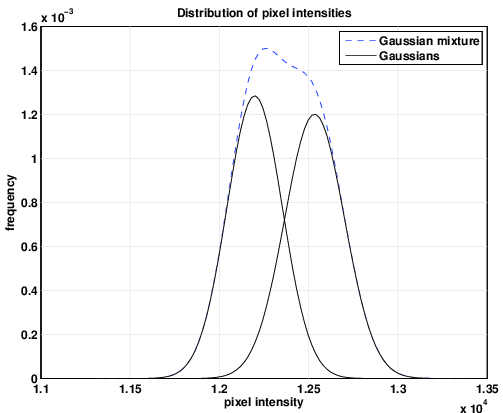
\includegraphics[width=0.5\textwidth]{figures/gaussians.png}
\caption{Density of a mixture of two normal distributions, whose means
  are the background and the fringe amplitudes, respectively.  }
\label{fig:gaussian_mixture_model}
\end{figure}

Thus the density function $f(x)$ of the intensity of an individual
pixel is modeled as follows
\begin{equation}
  f(x) = c_1\,e^{ -\frac{(x-\mu_1)^2}{2\sigma_1^2} }
  + c_2\,e^{ -\frac{(x-\mu_2)^2}{2\sigma_2^2} }.
\end{equation}

The means $\mu_1$ and $\mu_2$ ( $\mu_1 < \mu_2 = \mu_{1}+a$) are
proportional to the background amplitude and the fringe pattern
amplitude, respectively.  These values are used for normalization of
the background and fringe amplitudes before stacking.

The parameters of the two Gaussian components are estimated from the
density function of the pixel intensities by a nonlinear least squares
fit algorithm.  The algorithm requires as its input an estimated
density function.  Such an estimate is calculated in a preprocessing
step as a truncated Hermite series:
\begin{equation}
  f(x) \approx \sum_{n=0}^p \; c_n h_n\left(\frac{x - \mu}{\sigma}\right),
\end{equation}
where $h_n$ is the normalized Hermite function
\begin{equation}
  h_n(x) = {\pi}^{-\frac14} \,
  2^{-\frac{n}{2}} (n!)^{-\frac12} \, (\-1)^n \, e^{\frac{x^2\!\!}{2}} \,
  \frac{d^n}{dx^n}\left( e^{-x^2} \right),
\end{equation}
$\mu$ and $\sigma$ are, respectively, the sample mean and the sample
standard deviation of pixel intensities in the given image.  The
truncation parameter $p$ is found experimentally, $p = 20$ has been
sufficient so far.  The Hermite coefficients $c_n$ are computed as
follows
\begin{equation}
  c_n = \frac1{\sigma N}\; \sum_{i=1}^N h_n\left(\frac{I_i - \mu}{\sigma}\right),
\end{equation}
where the summation extends over all pixel intensities
$I_1, \ldots, I_{N}$, $N$ is the total number of pixels, and
$n = 0, \ldots, p$.

A detailed description of the algorithm can be found in
appendix~\ref{chap:algorithms:fringing}


\paragraph{Functions}
\label{fringe:algorithms:compute:functions}

The master fringe is computed using the following function

\begin{lstlisting}
cpl_error_code hdrl_fringe_compute(
        hdrl_imagelist          *  ilist_fringe, 
        const cpl_imagelist     *  ilist_obj,
        const cpl_mask          *  stat_mask, 
        const hdrl_parameter    *  collapse_params,
        hdrl_image              ** master, 
        cpl_image               ** contrib_map,
        cpl_table               ** qctable)
\end{lstlisting}

The output \verb+master+ and \verb+contrib_map+ products are filled
with the resulting master fringe and associated contribution map
images. The output \verb+qctable+ product contains the background
level (in table column \\ \verb+Background_level+) and the fringe
amplitude (in table column \verb+Fringe_amplitude+) computed by the
algorithm for each input image. The corresponding object data has to
be deleted by the user when not required any more.\\
Please note that if the background level and the fringe amplitude can
not be computed a warning is issued. Moreover, in this case a
background level of 0 and a fringe amplitude of 1 is assumed, i.e. the
original image is used in the following steps.

\paragraph{Inputs}
\label{fringe:algorithms:compute:inputs}

The list of images affected by fringes that should be combined to form
the master fringe is passed to the function with the hdrl imagelist
\verb+ilist_fringe+ input function-parameter.  If object masks are
needed to distinguish between sky and object pixels (very important!)
they can be passed with the cpl imagelist \verb+ilist_obj+ input
function-parameter.  Moreover, if a static mask is needed to
distinguish between regions with prominent and weak fringes it can be
passed with the cpl mask \verb+stat_mask+ input function-parameter.

Please note that the static mask \verb,stat_mask, and the object masks
\verb,ilist_obj, are optional input function-parameters, i.e. one can
pass NULL if no mask should be used.

The \verb+collapse_params+ parameter controls the collapsing algorithm
of the master fringe computation and is a \verb+hdrl_parameter+. Its
type defines the collapse method which is applied. Currently available
are the following collapsing parameter creation utilities:
\begin{itemize}\itemsep-1pt \parskip0pt \parsep0pt\small
\item \verb+hdrl_collapse_mean_parameter_create()+
\item \verb+hdrl_collapse_median_parameter_create()+
\item \verb+hdrl_collapse_weighted_mean_parameter_create()+
\item \verb+hdrl_collapse_sigclip_parameter_create(kappa_low, kappa_high, niter)+
\item \verb+hdrl_collapse_minmax_parameter_create(nlow, nhigh)+
\item \verb+hdrl_collapse_mode_parameter_create(histo_min, histo_max, bin_size,+\\\verb+mode_method, error_niter)+
\end{itemize}

Note that these parameters are dynamically allocated and must be
deleted when not needed.  For convenience HDRL provides preallocated
parameters for collapsing operations (e.g. \verb+HDRL_COLLAPSE_MEAN+)
which do not require any additional parameters. These can be used
anywhere a regular parameter can be used (deletion with
\verb+hdrl_parameter_delete+ has no effect on them). See
section~\ref{sec:imagelist:collapsing} for more details.

\paragraph{Outputs}
\label{fringe:algorithms:compute:outputs}

The result is a \verb+hdrl_image+ stored in the function-parameter
\verb+master+ containing the master fringe and its associated error as
well as an integer contribution map (\verb+contrib+) counting how many
values contributed to each pixel of the image. Moreover, the output
table \verb+qctable+ contains the derived background level in the
table column \verb+Background_level+ and the fringe amplitude in table
column \verb+Fringe_amplitude+ for each input image.


\subsubsection{Master fringe correction}
\label{fringe:algorithms:correct}

This algorithm scales and subtracts a master fringe from a sequence of
images.

\paragraph{Algorithm - short description}
\label{fringe:algorithms:correct:short}

The function subtracts a passed master fringe image
(\verb,masterfringe,) from a set of input images
(\verb,ilist_fringe,). The amplitude of the fringes is computed for
each input image and used to properly rescale the correction image
before subtraction.

The algorithm computes fringe amplitudes for each individual image by
a least squares fit of a linear combination of the estimated
master-fringe and a constant background.  Specifically, the $i$th
fringe $F_i$ is estimated as
\begin{equation}
  F_{i} = a_{i}F + b_{i},
\end{equation}
where $F$ is the estimated stacked master-fringe, and $b_i$ is a
constant representing the background.  The unknown constants $a_i$ and
$b_i$ are computed by a standard least squares fit preformed over the
unmasked pixels.

Moreover, different masks controlling the algorithm in different
stages can be passed to the hdrl function e.g. a static mask
(\verb,stat_mask,) to exclude regions where the fringe is weak -
sometimes essential for an accurate scaling estimation of noisy
images. The algorithm combines the bad pixel map (from
\verb,ilist_fringe),, the object mask (from \verb,ilist_obj,), and
static mask (\verb,stat_mask,) for the scaling computation of the
master fringe, but only uses the bad pixel map when subtracting the
master-fringe. The object mask and static mask are ignored in this
step. This ensures that the master fringe is properly subtracted (with
error propagation) in all regions not affected by the bad pixel mask.

Please note, that the function directly works on the passed hdrl
imagelist (\verb,ilist_fringe,) in order to save memory thus modifying
this imagelist i.e. removing the fringes directly from
\verb,ilist_fringe,. Moreover, the scaling factor derived and used in
this function is considered to be noiseless, i.e. the associated error
is supposed to be zero.

A detailed description of the algorithm can be found in
appendix~\ref{chap:algorithms:fringing}

\paragraph{Functions}
\label{fringe:algorithms:correct:functions}

The fringe correction is done by the following function

\begin{lstlisting}
cpl_error_code hdrl_fringe_correct(
        hdrl_imagelist          *  ilist_fringe, 
        const cpl_imagelist     *  ilist_obj,
        const cpl_mask          *  stat_mask, 
        const hdrl_image        *  masterfringe,
        cpl_table               ** qctable);
\end{lstlisting}

The function one-by-one scales and subtracts the passed master-fringe
image \verb,masterfringe, from the images stored in
\verb,ilist_fringe,. The output \verb+qctable+ product contains the
background level (in table column \verb+Background_level+) and the
fringe amplitude (in table column \verb+Fringe_amplitude+) computed by
the algorithm for each input image. The corresponding object data has
to be deleted by the user when not required any more.\\
Please note that if the background level and the fringe amplitude can
not be computed a warning is issued. Moreover, in this case a
background level of 0 and a fringe amplitude of 0 is assumed, i.e. no
correction will be applied to this image.



\paragraph{Inputs}
\label{fringe:algorithms:correct:inputs}


The list of images that should be fringe corrected by the master
fringe is passed to the function with the hdrl imagelist
\verb+ilist_fringe+ whereas the master-fringe is passed in the
\verb+masterfringe+ input function-parameter.

If object masks are needed to distinguish between sky and object
pixels (very important!)  they can be passed with the cpl imagelist
\verb+ilist_obj+ input function-parameter.  Moreover, if a static mask
is needed to distinguish between regions with prominent and weak
fringes it can be passed with the cpl mask \verb+stat_mask+ input
function-parameter.  Please note that the static mask \verb,stat_mask,
and the object masks \verb,ilist_obj, are optional input
function-parameters, i.e. one can pass NULL if no mask should be used.

\paragraph{Outputs}
\label{fringe:algorithms:correct:outputs}

The algorithm directly modifies the input hdrl images
\verb+ilist_fringe+ when performing the fringe correction, thus the
result is stored in the latter. Moreover, the output
table \verb+qctable+ contains the derived background level in the
table column \verb+Background_level+ and the fringe amplitude in table
column \verb+Fringe_amplitude+ for each input image.
